% NeurIPS 2026 Submission
% Working title: Constant Auxiliary Losses Considered Harmful
%
% Style file: neurips_2026.sty (download from neurips.cc before compiling)
% Anonymous submission mode active.

\documentclass{article}

% For submission (anonymous review):
\usepackage{neurips_2026}
% For preprint development (uncomment below, comment above):
% \usepackage[preprint]{neurips_2026}

\usepackage{amsmath}
\usepackage{amssymb}
\usepackage{mathtools}
\usepackage{amsthm}
\usepackage{booktabs}
\usepackage{graphicx}
\usepackage{subcaption}
\usepackage{hyperref}
\usepackage{cleveref}
\usepackage{algorithm}
\usepackage{algorithmic}
\usepackage{microtype}
\usepackage{xcolor}

\theoremstyle{plain}
\newtheorem{theorem}{Theorem}
\newtheorem{lemma}[theorem]{Lemma}
\newtheorem{proposition}[theorem]{Proposition}
\theoremstyle{definition}
\newtheorem{definition}[theorem]{Definition}
\theoremstyle{remark}
\newtheorem{remark}[theorem]{Remark}

\title{Constant Auxiliary Losses Considered Harmful:\\
A Cautionary Tale in Belief-Learning Multi-Agent Reinforcement Learning}

% Author block hidden for anonymous review.
% \author{
%   Vishnu Kadiyala \\
%   School of Computer Science\\
%   University of Oklahoma\\
%   \texttt{vishnupk@ou.edu}
%   \And
%   Mohammed Atiquzzaman \\
%   School of Computer Science\\
%   University of Oklahoma\\
%   \texttt{atiq@ou.edu}
% }

\begin{document}

\maketitle

\begin{abstract}
Attention-based belief encoders trained with constant-weight auxiliary
prediction losses targeting teammate future behavior appear in recent
cooperative multi-agent reinforcement learning (MARL) methods such as
BEPAL~\cite{huang2025bepal} and Dynamic Belief~\cite{zhai2023dynamic}.
We identify a directional gradient-interference pathology in this
design pattern under co-learning non-stationarity, building on Zhai et
al.'s independent observation that naively co-trained teammate-action
prediction can hurt decentralized policy learning. To isolate the
mechanism we construct VABL as a minimal architecture in the same
class and run a 7-configuration ablation across Overcooked, SMAX, and
MPE. On the
Overcooked headline ablation, the Full (attention + constant aux)
cell is the only one that exhibits late-training instability; the
pattern reproduces on SMAX but is absent on the simpler MPE
cooperative navigation, consistent with
Proposition~\ref{prop:variance}'s environment-dependent threshold. On
Overcooked, three gradient-targeted interventions all sever the
auxiliary-to-encoder pathway and converge to the no-aux regime; on
SMAX the same interventions reduce cross-seed variance but leave a
residual mean gap, which we flag as an open question. A gradient
decomposition reveals the auxiliary gradient is small in magnitude
relative to the policy gradient yet oscillates erratically in
direction, pointing to directional rather than magnitude-driven
interference. A 60-run architecture sweep reproduces the effect in
two of four attention-based actor configurations; mean pooling is
immune and critic-side auxiliary placement reverses the sign. We
additionally show that ``coordination collapse'' on Overcooked is
largely a training-budget artifact. For practitioners on
architectures in this class, any of $\lambda \leq 0.01$ or annealing,
stop-gradient on the belief into the auxiliary head, or critic-side
auxiliary placement suffices on Overcooked. Code, training logs, and
per-seed results for all 350{+} runs are available at
\url{https://anonymous.4open.science/r/aux-loss-considered-harmful}.
\end{abstract}


% ============================================================================
\section{Introduction}
\label{sec:intro}
% ============================================================================

Cooperative MARL on Overcooked is widely reported to collapse after
reaching strong peak reward during training: MAPPO by
76\%~\cite{yu2022surprising}, AERIAL by
100\%~\cite{phan2023attention}, with communication-based methods
showing similar instability~\cite{das2019tarmac, sukhbaatar2016commnet}.
These reports have motivated auxiliary prediction
losses~\cite{jaderberg2016reinforcement}, attention-based belief
encoders~\cite{phan2023attention}, and explicit communication channels
as stabilization mechanisms. The resulting design pattern, a shared
encoder trained jointly with a policy loss and a constant-weight
auxiliary prediction loss, is now widespread beyond MARL, appearing
in world models~\cite{hafner2023mastering}, multi-task
RL~\cite{jaderberg2016reinforcement}, and self-supervised
representation learning~\cite{schwarzer2021dataefficient}. We find
most of the reported Overcooked collapse to be a training-budget
artifact: collapse drops from $\sim$46\% at 500K to $<$3\% at 10M, and
MAPPO, TarMAC, and CommNet all converge stably by 10M
(Section~\ref{sec:budget}).

\textbf{The design pattern and isolating its mechanism.}
BEPAL~\cite{huang2025bepal} and Dynamic Belief~\cite{zhai2023dynamic}
combine attention-based belief encoders with constant-weight
teammate-future-prediction aux; Dynamic Belief's Static-Belief
ablation independently reports that naive co-training drops success
below no-aux, attributed to teammate non-stationarity. We construct
\textbf{VABL}, a minimal architecture in this design-pattern class
with a cleanly separable aux pathway. In our 7-config ablation on
Overcooked AA at 10M, the attention + constant-aux cell is the only
one with late-training instability while every configuration reaches
the same Best ceiling. The pathology reproduces on Cramped Room and
SMAX but is absent on MPE simple\_spread, consistent with
Proposition~\ref{prop:variance}'s environment-dependent threshold.
Three gradient-targeted interventions ($\lambda$-annealing,
stop-gradient on the belief into the aux head, and both combined)
converge to a recovered regime statistically equivalent to removing
aux. A CIFAR-100 cross-domain test finds the pathology absent in
supervised learning, narrowing it to MARL co-learning non-stationarity.

Our contributions: \textbf{(1)}~a directional
gradient-interference pathology in the attention + constant-auxiliary
design pattern used by BEPAL~\cite{huang2025bepal} and
Dynamic Belief~\cite{zhai2023dynamic}, isolated under controlled
ablation in VABL, with
environment-dependence (present on Overcooked and SMAX, absent on MPE);
\textbf{(2)}~a descriptive stochastic model
(Proposition~\ref{prop:variance}, bound scaling with
$\mathrm{tr}(\Sigma_\varepsilon)/\lambda_{\min}(H)$) and gradient
decomposition showing the mechanism is directional, not
magnitude-driven; \textbf{(3)}~three gradient-targeted fix paths
($\lambda{\leq}0.01$ or annealing, stop-gradient on the belief, or
critic-side auxiliary placement) that all sever the aux-to-encoder
pathway and recover to the no-aux regime on Overcooked (on SMAX they
reduce variance but leave a residual mean gap; see \S\ref{sec:budget}),
generalized in a 60-run architecture sweep (Table~\ref{tab:arch_sweep}); \textbf{(4)}~evidence
that the much-reported Overcooked coordination collapse is largely a
training-budget artifact, plus a reproducible 350{+}-run, 5-seed
benchmark with anonymized code at
\url{https://anonymous.4open.science/r/aux-loss-considered-harmful}.


% ============================================================================
\section{Related Work}
\label{sec:related}
% ============================================================================

\paragraph{Auxiliary losses in RL.}
UNREAL~\cite{jaderberg2016reinforcement} pioneered auxiliary tasks;
subsequent work uses world-model
losses~\cite{hafner2023mastering}, self-predictive
representations~\cite{schwarzer2021dataefficient,fang2024predictive},
and contrastive objectives~\cite{laskin2020curl}. Theoretical analyses
of auxiliary-task
dynamics~\cite{lyle2021effect,voelcker2024selfprediction} cover TD and
latent self-prediction; \cite{du2018adapting,lin2019adaptive} argue
constant weights are suboptimal.
\cite{moalla2024norepnotrust} document on-policy PPO representation
collapse under non-stationarity; \cite{chua2024successor} show
successor-feature losses collapse basis features to cosine-to-1,
resolved by stop-gradient in the reward loss. In MARL,
XP-MARL~\cite{xu2024xpmarl} uses auxiliary prioritization for
non-stationarity. BEPAL~\cite{huang2025bepal} and Dynamic
Belief~\cite{zhai2023dynamic} directly instantiate the design pattern
we study (attention-based belief encoder + fixed-weight
teammate-future-prediction aux). Zhai et al.'s Static-Belief ablation
(their Table~2) independently reports that naively co-trained
teammate-action prediction drops Traffic Junction success from
$73.4\%$ (baseline) to $71.9\%$, attributed to teammate
non-stationarity; their fix is meta-learned dynamic context. Our
study isolates the same failure mode in a controlled ablation,
identifies directional gradient interference as the mechanism, and
characterizes three gradient-pathway interventions.

\paragraph{Attention in MARL.}
AERIAL~\cite{phan2023attention} uses QMIX-based attention over
teammate hidden states (no auxiliary head);
MAAC~\cite{iqbal2019actor} places attention in the centralized critic;
MAT~\cite{wen2022mat} uses an encoder-decoder for centralized policy
learning. None pair attention-based \emph{decentralized} belief
encoding with the specific constant-weight teammate-future-prediction
auxiliary loss that our study characterizes.

\paragraph{Stop-gradient in SSL and RL.}
BYOL~\cite{grill2020bootstrap}, SimSiam~\cite{chen2021exploring}, and
DINO~\cite{caron2021emerging} use stop-gradient to prevent
representation collapse in self-supervised learning; Chua et
al.~\cite{chua2024successor} apply the same mechanism to basis features
in successor-feature learning. Our stop-gradient fix path is analogous:
it prevents the auxiliary loss from destabilizing the belief encoder
via gradient interference.

\paragraph{Gradient interference.}
PCGrad~\cite{yu2020gradient}, GradNorm~\cite{chen2018gradnorm},
HyperMARL~\cite{tessera2025hypermarl}, and multi-timescale
learning~\cite{nekoei2023dealing} project, reweight, or decouple
gradients by magnitude or across agents. Direction-oriented
MOO~\cite{xiao2023sdmgrad,zhang2025mgda,patapati2025graphcoloring}
regularizes the conflict-avoidant direction or schedules by cosine
interference. In offline MARL, \cite{tilbury2024coordination} identify
a distinct directional pathology where data-mean-biased best responses
steer joint gradients away from the optimum. Our pathology is
intra-agent, \emph{directional} rather than magnitude-driven
(aux gradient $<25\%$ of policy magnitude but erratically oriented
under co-learning), and environment-dependent. Existing frameworks
target none of these signatures.

\paragraph{Coordination collapse.}
Overcooked~\cite{carroll2019utility} is widely used for cooperative
MARL~\cite{huh2024multiagent} with prior reports of severe
degradation~\cite{yu2022surprising,rashid2020monotonic,das2019tarmac};
cooperative MARL also exhibits named pathologies such as relative
overgeneralization~\cite{wei2016lenient} and deep RL's late-training
capacity loss~\cite{lyle2022capacity}. Recent benchmarking shows
algorithm rankings depend sharply on training budget:
\cite{formanek2024mirage} find 75\% of offline MARL SOTA claims
reverse under standardized budgets, and \cite{papadopoulos2025extended}
report high cross-seed variance on Overcooked at 40M--100M steps;
BenchMARL~\cite{bettini2024benchmarl} proposes standardized
infrastructure as remedy. At 10M steps most reported ``collapse'' is
insufficient training; the residual instability we identify is
distinct and gradient-mediated.


% ============================================================================
\section{Background: Attention-Based Belief Learning}
\label{sec:background}
% ============================================================================

The design pattern we investigate, attention-based belief encoders
trained with constant-weight auxiliary prediction losses targeting
teammate future behavior, has two recent published instances.
BEPAL~\cite{huang2025bepal} uses a shared LSTM with attention over
teammate messages and belief-decoder heads predicting teammates'
future motion and reward with fixed weights; Dynamic
Belief~\cite{zhai2023dynamic} uses soft attention over episode history
with a VAE-based head predicting teammates' future actions with fixed
weights. These sit within the broader family of world-model and
self-predictive architectures that use constant auxiliary
weights~\cite{hafner2023mastering,schwarzer2021dataefficient,jaderberg2016reinforcement}.
We construct \textbf{VABL} as a minimal architecture in this class,
operating on cooperative Dec-POMDPs~\cite{oliehoek2016concise}, and
chosen so that attention, the auxiliary loss, and the gradient flow
between them can be manipulated independently.

\paragraph{Belief update.}
Each agent $i$ maintains a recurrent latent belief $b_t^i \in
\mathbb{R}^{d_h}$, updated at each timestep from (i) an observation
embedding $\phi_\theta(o_t^i) \in \mathbb{R}^{d_e}$ and (ii) a social
context vector $c_t^i \in \mathbb{R}^{d_e}$ aggregated from observable
teammate actions:
\begin{equation}
    b_t^i = \mathrm{GRU}\left(
        [\phi_\theta(o_t^i) \| c_t^i],\; b_{t-1}^i
    \right),
\end{equation}
where $\mathrm{GRU}$ denotes a gated recurrent unit~\cite{cho2014gru}.

\paragraph{Attention context.}
The social context is computed via multi-head attention~\cite{vaswani2017attention} over action embeddings
of visible teammates:
\begin{equation}
    c_t^i = \mathrm{MHA}\left(
        \mathrm{query} = W_q b_{t-1}^i, \quad
        \mathrm{keys/values} = \{\psi_\theta(a_{t-1}^j) + e_j\}_{j \neq i}
    \right),
\end{equation}
where $\psi_\theta$ is an action encoder, $e_j$ is a learnable identity
embedding for teammate $j$, and the attention is masked by a visibility
indicator $m_t^{i \leftarrow j} \in \{0,1\}$. When no attention is used
(the mean-pooling ablation), $c_t^i$ is the unweighted average of visible
teammate action embeddings.

\paragraph{Policy and auxiliary heads.}
The policy $\pi_\theta(a_t^i \mid b_t^i)$ is a linear head on the belief.
The auxiliary predictor $\hat{\pi}_\varphi(\cdot \mid b_t^i)$ is a 2-layer
MLP that predicts each visible teammate's next action from the current
belief, trained with cross-entropy:
\begin{equation}
    \mathcal{L}_{\mathrm{aux}}^i = \mathbb{E}\left[
        \sum_{j \neq i} m_{t+1}^{i \leftarrow j}\,
        \mathrm{CE}(\hat{\pi}_\varphi(\cdot \mid b_t^i),\, a_{t+1}^j)
    \right].
\end{equation}

\paragraph{Training objective.}
The total loss combines a PPO policy gradient~\cite{schulman2017ppo}, a centralized value loss, entropy
regularization, and the auxiliary loss:
\begin{equation}
    \mathcal{L} = \mathcal{L}_{\mathrm{PPO}} +
    c_v \mathcal{L}_{\mathrm{value}} +
    c_e \mathcal{L}_{\mathrm{entropy}} +
    \lambda \sum_i \mathcal{L}_{\mathrm{aux}}^i,
\end{equation}
where $\lambda = 0.05$ is the auxiliary loss weight. In the standard
configuration, $\lambda$ is held constant throughout training.

\paragraph{Gradient pathway.} The auxiliary loss gradient flows
through the belief $b_t^i$ into the attention mechanism, GRU, and
observation encoder $\phi_\theta$. Section~\ref{sec:results} identifies
this pathway as the source of the late-training instability.


% ============================================================================
\section{Descriptive Model: Directional Interference}
\label{sec:theory}
% ============================================================================

We develop a minimal analytical model that predicts the empirical findings.
The key insight is that the pathology arises not from the \emph{magnitude}
of the auxiliary gradient but from its \emph{directional variance} under
co-learning non-stationarity.

\paragraph{Gradient decomposition near convergence.}
Near a local optimum $\theta^*$, the policy loss is approximately quadratic
with Hessian $H$, giving policy gradient $\nabla_\theta L_{\mathrm{policy}}
= H(\theta - \theta^*)$, which shrinks as $\theta \to \theta^*$. The
auxiliary gradient $g_{\mathrm{aux}}(t) = \lambda \nabla_\theta
L_{\mathrm{aux}}(\theta; \pi_j^{(t)})$ depends on teammate $j$'s current
policy $\pi_j^{(t)}$, which is non-stationary under co-learning.

\paragraph{Noise decomposition.}
We decompose $g_{\mathrm{aux}}(t) = \bar{g}_{\mathrm{aux}} + \varepsilon(t)$
into a mean component and zero-mean noise with covariance
$\Sigma_\varepsilon$. The noise $\varepsilon(t)$ arises specifically
from co-learning
non-stationarity~\cite{hernandezleal2017survey, nekoei2023dealing}: if
teammate $j$'s policy were frozen, $\varepsilon \to 0$. Prior work
tackles this non-stationarity through multi-timescale learning rather
than through a gradient-level analysis of how auxiliary objectives
propagate into shared encoders.

\paragraph{Stochastic dynamics.}
Centering around the effective fixed point $\theta^*_{\mathrm{eff}} =
\theta^* - H^{-1}\bar{g}_{\mathrm{aux}}$, the displacement $\delta(t) =
\theta(t) - \theta^*_{\mathrm{eff}}$ evolves as:
\begin{equation}
    \delta(t{+}1) = (I - \alpha H)\,\delta(t) - \alpha\,\varepsilon(t),
    \label{eq:dynamics}
\end{equation}
a linear stochastic system driven by the directional noise of the auxiliary
gradient.

Intuitively, late-training parameter variance grows with the
auxiliary-gradient directional noise $\Sigma_\varepsilon$ (numerator)
and shrinks with the minimum policy-loss curvature $\lambda_{\min}(H)$
(denominator); a flatter landscape amplifies the noise. The
proposition is \emph{descriptive}, relating two measurable quantities
under a simplifying assumption.

\begin{proposition}[Steady-state variance; descriptive linear model]
\label{prop:variance}
Consider the linearized dynamics of Eq.~\eqref{eq:dynamics} with
noise $\varepsilon(t)$ (Cov $= \Sigma_\varepsilon$, treated as
i.i.d.\ for tractability) and spectral radius $\rho(I - \alpha H) < 1$.
Given these primitives, the steady-state parameter variance satisfies:
\begin{equation}
    \mathbb{E}[\|\delta\|^2]
    \;\propto\;
    \frac{\alpha^2 \,\mathrm{tr}(\Sigma_\varepsilon)}
         {\lambda_{\min}(H)}.
    \label{eq:variance_bound}
\end{equation}
\end{proposition}

\textit{Assumptions and scope.} This is a descriptive model, not a
first-principles prediction. We treat $\Sigma_\varepsilon$ as empirical
(Figure~\ref{fig:gradients}) rather than derived; quadratic loss and
i.i.d.\ noise simplify real PPO. A synthetic experiment with prescribed
$H$ and $\Sigma_\varepsilon$ recovers the bound
(Appendix~\ref{app:synthetic}). The qualitative implications explain
why the fix paths work: each severs the aux-to-encoder gradient pathway,
driving $\Sigma_\varepsilon \to 0$ in the encoder subspace.

\begin{proof}[Proof sketch]
The steady-state covariance satisfies the discrete Lyapunov equation
$\Sigma_\delta = A \Sigma_\delta A^T + \alpha^2 \Sigma_\varepsilon$
with $A = I - \alpha H$. Diagonalizing yields
$\mathrm{tr}(\Sigma_\delta) = \alpha^2 \sum_i
\sigma_{\varepsilon,i}^2 / (2\alpha h_i - \alpha^2 h_i^2)$, dominated by
$\lambda_{\min}(H)$. Full derivation in Appendix~\ref{app:proof}.
\end{proof}

\paragraph{Qualitative consistencies with experiment.}
Five qualitative implications of Eq.~\eqref{eq:variance_bound} align
with our experiments (post-hoc consistencies, not \emph{a priori}
predictions):
(i)~attention amplifies $\Sigma_\varepsilon$ via multiplicative
belief-query coupling, matching Full VABL's std $8.55$ vs.\ $1.86$--$3.72$
for alternatives;
(ii)~driving $\Sigma_\varepsilon \to 0$ in the encoder subspace, via
annealing or stop-gradient, recovers stability (B\_anneal $473.66$,
B\_stopgrad $471.60$ $\approx$ A\_no\_aux $473.45$; B\_stopgrad's std
$2.13$ is smallest);
(iii)~fixed supervised targets drive $\Sigma_\varepsilon \to 0$
naturally, matching CIFAR-100's $<0.5$-point aux effect
(Appendix~\ref{app:vision});
(iv)~complex co-learning increases $\Sigma_\varepsilon$ above threshold,
present on Overcooked and SMAX but absent on MPE;
(v)~smaller $\lambda$ should reduce
$\mathrm{tr}(\Sigma_\varepsilon)$, but only partially: $\lambda{=}0.05$
is pathological (std $8.55$) and $\lambda{=}0.01$ stable (std $1.67$),
while $\lambda{=}0.001$ (std $6.37$) does not improve further. We read
this as a sweet spot rather than a monotonic threshold: the aux signal
both regularizes representations and introduces directional noise, and
the optimum balances the two.

Figure~\ref{fig:gradients} plots the gradient decomposition on Full
VABL (AA). The directional instability persists even as the auxiliary
gradient decreases across training, confirming a directional rather
than magnitude-driven mechanism.

\begin{figure}[t]
\centering
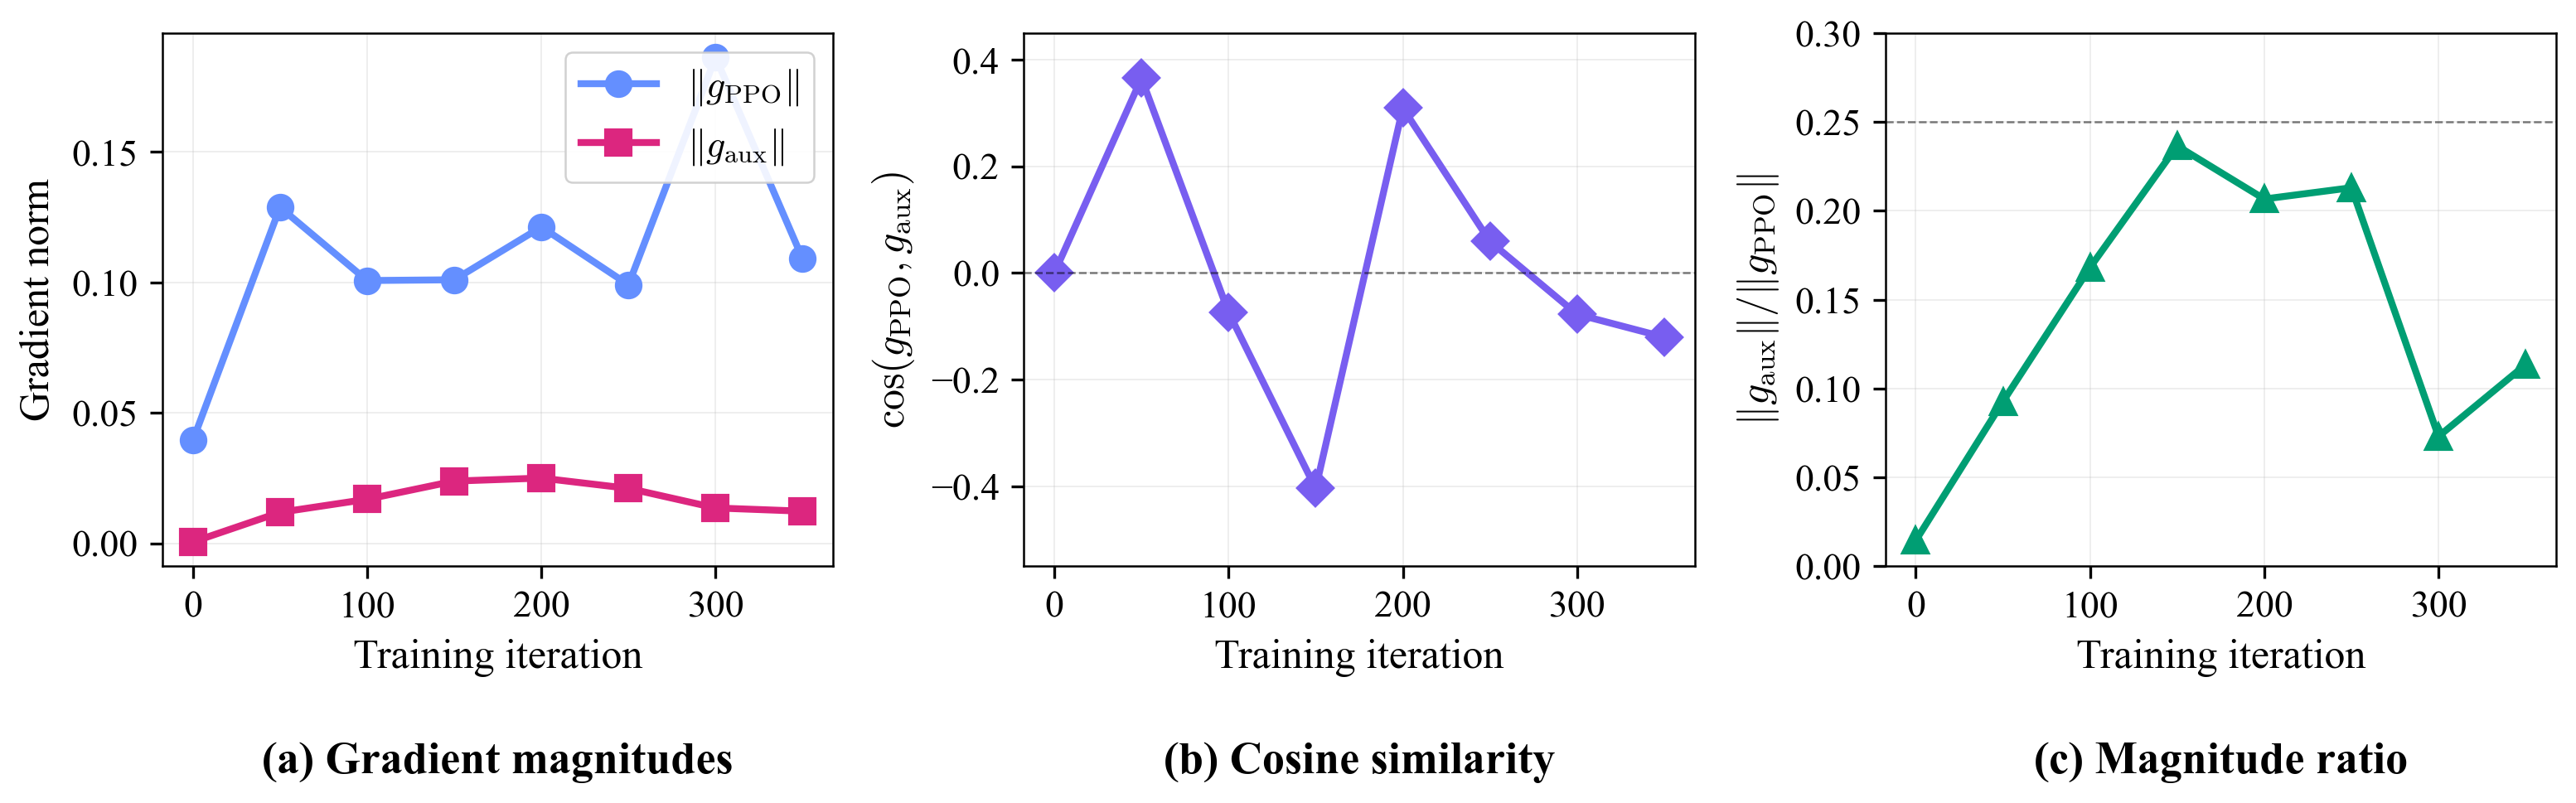
\includegraphics[width=\columnwidth]{figures/neurips/f6_gradients.pdf}
\caption{Gradient decomposition over training for Full VABL on AA (seed~0 shown; pattern consistent across all 5 seeds with cosine range $[-0.47, +0.33]$). \textbf{(a)}~The PPO gradient (blue) stays large while the auxiliary gradient (red) \emph{decreases}. \textbf{(b)}~Cosine similarity oscillates erratically, confirming directional interference. \textbf{(c)}~The magnitude ratio is always $< 0.25$; the pathology is not magnitude-driven.}
\label{fig:gradients}
\end{figure}


% ============================================================================
\section{Methodology}
\label{sec:method}
% ============================================================================

\subsection{Ablation Matrix and Fix-Path Interventions}
We run VABL in a $2 \times 2$ ablation over attention vs.\ mean
pooling and auxiliary loss on ($\lambda = 0.05$ constant) vs.\ off,
yielding \textbf{Full} (attn+aux), \textbf{No Attention}, \textbf{No
Aux}, and \textbf{Neither}. Three gradient-only interventions on
Full: \textbf{Anneal} (linearly decay $\lambda$ from $0.05$ to $0$
over the first 50\% of training), \textbf{Stop-gradient}
(\texttt{stop\_gradient} on $b_t^i$ before the aux head; aux MLP
still trains but gradients do not reach the encoder), and
\textbf{Anneal + stop-gradient} (both combined).

\subsection{Environments}
We evaluate three environment families.
\textbf{Overcooked}~\cite{carroll2019utility}: layouts \emph{Asymmetric
Advantages} and \emph{Cramped Room}, 2 agents, horizon 400, 25{,}024
episodes ($\approx$10M env steps), 64 vectorized envs via JAX
\texttt{vmap}.
\textbf{MPE simple\_spread}~\cite{lowe2017multi}: 3 symmetric
agents, horizon 25, 100K episodes ($\approx$2.5M steps).
\textbf{SMAX 3v3}~\cite{rutherford2024jaxmarl}: 3 allies vs.\ 3
heuristic enemies, horizon 100, 50K episodes ($\approx$5M steps). SMAX
covers both original SMAC~\cite{samvelyan2019starcraft} and SMAC
v2~\cite{ellis2023smacv2} scenarios, testing a fundamentally different
coordination domain (tactical combat vs.\ cooking/navigation).

\subsection{Baselines}

We compare against four methods spanning three paradigms:
\textbf{MAPPO}~\cite{yu2022surprising} (decentralized policy gradient),
\textbf{TarMAC}~\cite{das2019tarmac} (targeted explicit communication),
\textbf{CommNet}~\cite{sukhbaatar2016commnet} (broadcast communication), and
\textbf{AERIAL}~\cite{phan2023attention} (attention over teammate hidden
states). All baselines are reimplemented in JAX~\cite{bradbury2018jax} using the
JaxMARL framework~\cite{rutherford2024jaxmarl} and trained with the same
hyperparameters, vectorized environment wrapper, and evaluation protocol.

\subsection{Cross-Domain Test}

To test whether the pathology generalizes beyond MARL, we replicate the
$2 \times 2$ ablation on CIFAR-100~\cite{krizhevsky2009learning} image
classification with a small Vision
Transformer~\cite{dosovitskiy2020image} (4 layers, 192 dim, 4 heads,
patch size 4) and a RotNet auxiliary head (4-way rotation
prediction)~\cite{gidaris2018unsupervised}. The auxiliary loss uses the
same $\lambda = 0.05$ constant weight.

\subsection{Metrics}

\begin{itemize}
    \item \textbf{Best}: maximum episode reward (or test accuracy) achieved
    during training.
    \item \textbf{Final50} (MARL) / \textbf{Final5} (vision): mean of the
    last 50 episodes (or last 5 epochs), capturing the policy's stable
    convergence level.
    \item \textbf{Collapse \%}: $({\mathrm{Best} - \mathrm{Final}}) /
    {\mathrm{Best}} \times 100$.
    \item We report mean $\pm$ population standard deviation over 5 random
    seeds for all MARL experiments, and Cohen's $d$~\cite{cohen1988statistical}
    for effect sizes.
\end{itemize}


% ============================================================================
\section{Results}
\label{sec:results}
% ============================================================================

\subsection{A Related Observation in AERIAL}
\label{sec:aerial_observation}

Independent of our design-pattern study, our actor-critic port of
AERIAL~\cite{phan2023attention} (attention over teammate hidden states,
no aux head) exhibits a consistent Best$\to$Final50 drop of $\sim$15
points on 4 of 5 seeds on Overcooked AA at 10M
(Table~\ref{tab:aerial_per_seed}). We do not claim our mechanism
explains this: AERIAL has no auxiliary prediction head, so the
aux-to-encoder pathway we isolate in VABL is not present. The origin
of AERIAL's drop is an open question distinct from the design-pattern
pathology our main study characterizes.

\begin{table}[h]
\centering
\caption{Per-seed AERIAL trajectories on Overcooked Asymmetric
Advantages (10M steps). Four of five seeds show the characteristic
pattern: reach a peak of $\sim$482, then drift down $12$--$21$ points
by end of training. The fifth seed fails to converge at all,
plateauing at $\sim$360 from roughly $25\%$ of training onward. The
four healthy seeds average a $15.5$-point late-training drop, larger
than Full VABL's $11.6$ (Table~\ref{tab:ablation}, Group~A).}
\label{tab:aerial_per_seed}
\small
\begin{tabular}{lcccc}
\toprule
\textbf{Seed} & \textbf{Peak} & \textbf{Peak position} & \textbf{Final50} & \textbf{Drop} \\
\midrule
0 & 476.6 & 59\% & 460.1 & 16.5 \\
1 & 361.5 & 100\% & 360.3 & 1.2$^\ddagger$ \\
2 & 481.4 & 79\% & 468.5 & 12.9 \\
3 & 478.0 & 42\% & 457.4 & 20.6 \\
4 & 478.2 & 65\% & 466.2 & 12.0 \\
\midrule
\textit{4 healthy seeds (mean $\pm$ std)} & \textit{$478.6 \pm 1.7$} & -- & \textit{$463.0 \pm 4.4$} & \textit{$15.5 \pm 3.3$} \\
\textit{All 5 seeds (mean $\pm$ std)} & \textit{$455.1 \pm 46.9$} & -- & \textit{$442.5 \pm 41.3$} & \textit{$12.6 \pm 6.6$} \\
\bottomrule
\end{tabular}

\vspace{2pt}
{\footnotesize $^\ddagger$Seed 1 never converged (plateaued near
$360$); the reported ``drop'' reflects no real peak. Our
instability claims refer to the 4 healthy seeds; both aggregates
are shown for transparency.}
\end{table}

Our VABL study instantiates the attention +
teammate-future-prediction-aux design pattern of
BEPAL~\cite{huang2025bepal} and Dynamic Belief~\cite{zhai2023dynamic},
and admits clean aux-pathway ablation. AERIAL's drop magnitude is
comparable to Full VABL's ($11.6 \pm 7.2$, \S\ref{sec:pathology}) but
its origin is distinct and we do not claim to explain it.

\subsection{Isolating the Pathology in VABL}
\label{sec:pathology}

\begin{table}[t]
\centering
\caption{7-configuration ablation on Overcooked Asymmetric Advantages (10M steps, 5 seeds). Group~A: $2{\times}2$ ablation over attention and auxiliary loss. Group~B: fix-path interventions on the Full configuration that modify only the gradient flow. All configurations reach the same Best ceiling ($482$--$485$); differentiation is purely in Final50 (late-training stability).}
\label{tab:ablation}
\small
\setlength{\tabcolsep}{3pt}
\begin{tabular}{lcccccc}
\toprule
\textbf{Configuration} & \textbf{Attn} & \textbf{Aux} & \textbf{Best} & \textbf{Final50} & \textbf{std} & \textbf{$d$} \\
\midrule
\multicolumn{7}{c}{\textit{Group A: Ablation}} \\
\midrule
Full (attn + aux) & \checkmark & \checkmark & 483.8 & 463.21 & \textbf{8.55} & -- \\
Neither (mean only) & -- & -- & 482.6 & 469.70 & 3.72 & 0.88 \\
No Attention (mean + aux) & -- & \checkmark & 483.8 & 471.76 & 1.86 & 1.24 \\
No Aux (attn only) & \checkmark & -- & 484.4 & \textbf{473.45} & 3.62 & \textbf{1.40} \\
\midrule
\multicolumn{7}{c}{\textit{Group B: Fix Paths (Full + gradient intervention)}} \\
\midrule
+ Anneal ($\lambda \to 0$) & \checkmark & \checkmark$^*$ & 484.4 & 473.66 & 3.59 & 1.43 \\
+ Stop-gradient & \checkmark & \checkmark$^\dagger$ & 482.6 & 471.60 & \textbf{2.13} & 1.20 \\
+ Both & \checkmark & \checkmark$^{*\dagger}$ & 484.4 & 472.35 & 2.21 & 1.31 \\
\bottomrule
\end{tabular}

\vspace{2pt}
{\footnotesize Cohen's $d$ is vs.\ Full. $^*$Aux $\lambda$ linearly decayed $0.05 \to 0$ over first 50\% of training. $^\dagger$\texttt{stop\_gradient} on belief into aux head.}
\end{table}

\begin{figure}[t]
\centering
\begin{subfigure}[b]{0.48\textwidth}
\centering
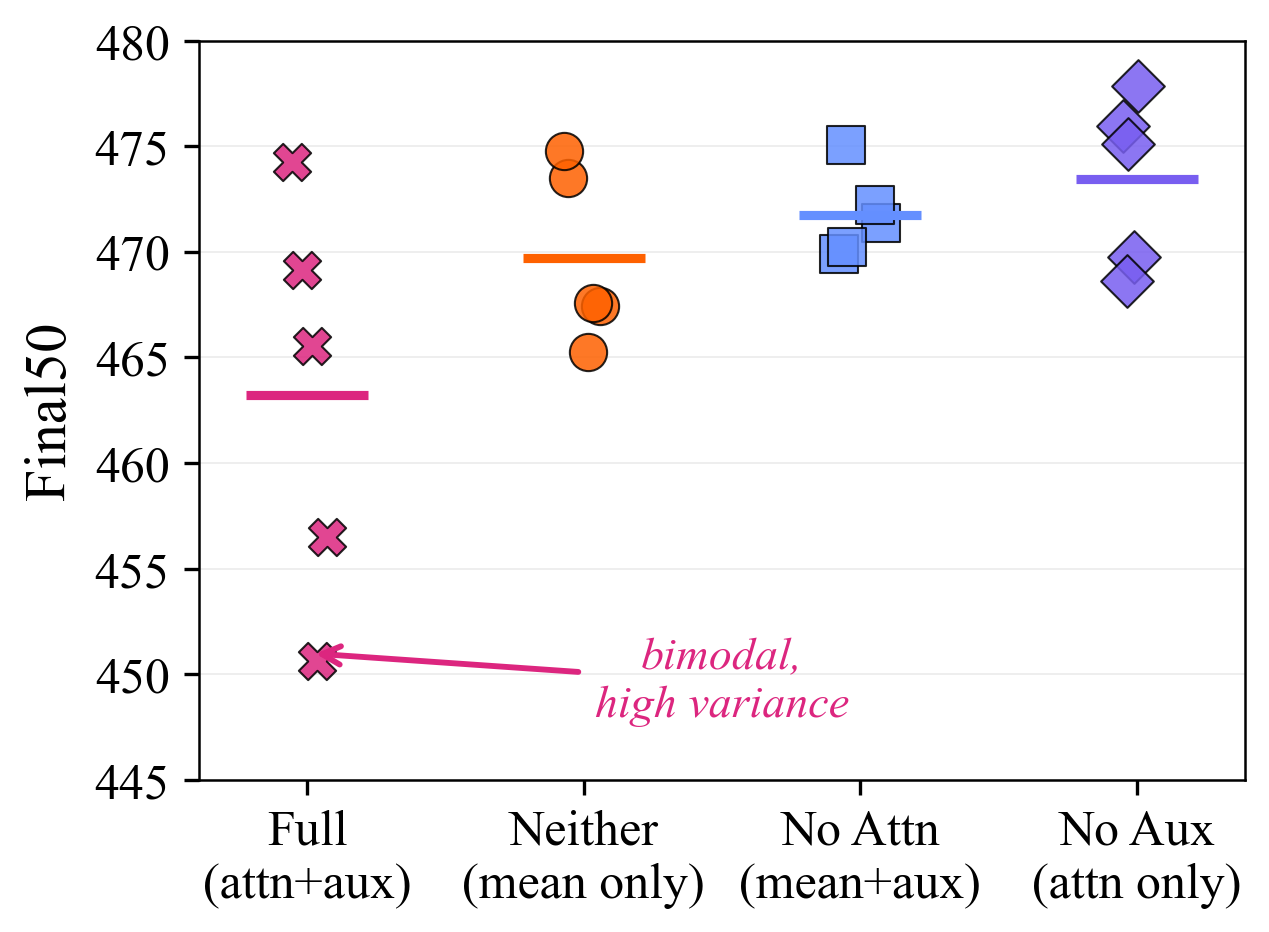
\includegraphics[width=\textwidth]{figures/neurips/f1_dotplot.pdf}
\caption{Per-seed Final50.}
\label{fig:dotplot}
\end{subfigure}
\hfill
\begin{subfigure}[b]{0.48\textwidth}
\centering
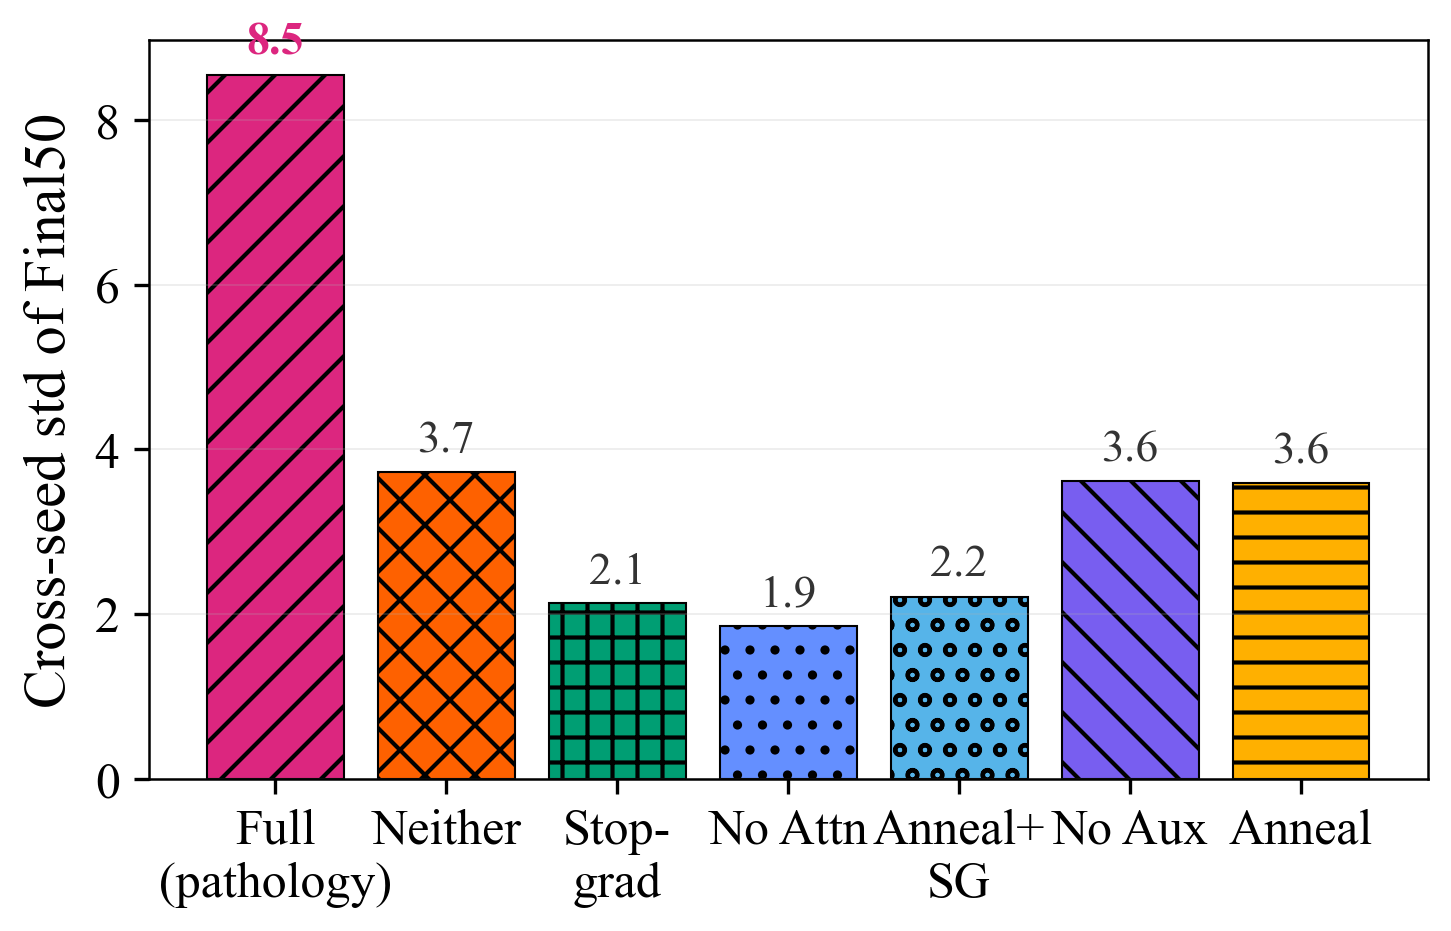
\includegraphics[width=\textwidth]{figures/neurips/f2_variance.pdf}
\caption{Cross-seed std across 7 configurations.}
\label{fig:variance}
\end{subfigure}
\caption{Cross-seed dispersion on Overcooked AA (10M steps, 5 seeds). \textbf{(a)}~Full VABL (magenta) has cross-seed std of $8.55$ ($2$--$5\times$ larger than alternatives); individual seeds drift $4$--$23$ points below their own peaks; horizontal lines show means. \textbf{(b)}~Std is monotonic in residual auxiliary gradient flow: full flow (Full) $\to$ phased-out (Anneal) $\to$ severed (Stop-grad, No Aux). Marker shapes and hatching vary for grayscale readability.}
\label{fig:dispersion}
\end{figure}

Table~\ref{tab:ablation} presents the 7-configuration ablation on
Overcooked AA at 10M steps. Only the Full (attention + constant aux)
configuration exhibits the pathology: Final50 is significantly lower
than every alternative (Cohen's $d \geq 0.88$) with $2$--$5\times$
higher cross-seed std, while all seven configurations reach the same
Best ceiling. The $2{\times}2$ interaction is clean: neither attention
alone nor the auxiliary loss alone causes the pathology; the instability
requires \emph{both} (full interaction in Appendix~\ref{app:tables}).

\subsection{Convergent Fix Paths}
\label{sec:fixes}

The three fix paths in Table~\ref{tab:ablation} (Group~B) all converge
to Final50 in $[471.60, 473.66]$, a 2.06-point spread smaller than the
seed envelope of any individual configuration, and statistically
equivalent to removing the auxiliary loss entirely (A\_no\_aux:
$473.45$). All three interventions intervene on the same pathway,
severing auxiliary gradient flow into the attention-based belief
encoder: annealing removes it over time, stop-gradient cuts it at its
source, and the combined intervention does both. The convergence to
the no-aux regime therefore identifies the aux-to-encoder gradient
pathway as the \emph{necessary conduit} for the pathology, rather than
confirming a specific functional form for how interference is
generated. Stop-gradient is the tightest of the three in that it
modifies \emph{only} the gradient flow (not the architecture, loss
function, forward pass, or reward signal) and reduces the cross-seed
standard deviation from $8.55$ to $2.13$, a $4\times$ reduction.

\subsection{Cross-Layout Generalization}
\label{sec:cramped}

\begin{table}[t]
\centering
\caption{Cross-layout generalization on Overcooked Cramped Room (10M steps, 5 seeds). All methods saturate at Best~$= 417$; differentiation is purely in Final50. The pathology reproduces with an even larger effect size (Cohen's $d = 5.06$).}
\label{tab:cramped}
\small
\begin{tabular}{lcccc}
\toprule
\textbf{Configuration} & \textbf{Final50} & \textbf{std} & \textbf{$d$ vs Full} & \textbf{95\% CI on $d$} \\
\midrule
Full (attn + aux) & 409.70 & 1.41 & -- & -- \\
No Attention (mean + aux) & 411.05 & 2.57 & $+0.58$ & $[-0.75, +2.35]$ \\
Neither (mean only) & 416.02 & 1.33 & $+4.13$ & $[+2.43, +8.32]$ \\
No Aux (attn only) & \textbf{416.18} & \textbf{0.79} & $\mathbf{+5.07}$ & $[+3.04, +10.74]$ \\
\bottomrule
\end{tabular}
\end{table}

The pathology reproduces on Cramped Room with a larger effect size
(Cohen's $d = 5.07$ vs. No Aux, 95\% parametric bootstrap CI
$[+3.04, +10.74]$; see Appendix~\ref{app:tables}). The auxiliary loss
is harmful regardless of whether attention is used, but the effect is
strongest in Full. The No~Attention comparison CI crosses zero, matching
the AA pattern where non-attention cells are harder to resolve at $n=5$.

\subsection{The Training-Budget Artifact}
\label{sec:budget}

\begin{table}[t]
\centering
\caption{6-method benchmark at 10M steps (5 seeds each). VABL uses the best ablation config (No Aux = attention only). Communication-based methods (TarMAC, CommNet) dominate in mean reward but with $30{\times}$ higher cross-seed variance than VABL. On Cramped Room, all methods saturate at the same ceiling. These baselines establish the training-budget artifact finding, since no method collapses at 10M, and are \emph{not} controls for the directional-interference pathology, which requires the attention + constant-auxiliary-loss design pattern that only VABL and AERIAL embody among methods evaluated.}
\label{tab:benchmark}
\small
\setlength{\tabcolsep}{3pt}
\begin{tabular}{lccccc}
\toprule
 & & \multicolumn{2}{c}{\textbf{Asymm.\ Advantages}} & \multicolumn{2}{c}{\textbf{Cramped Room}} \\
\cmidrule(lr){3-4} \cmidrule(lr){5-6}
\textbf{Method} & \textbf{Comm?} & \textbf{Final50} & \textbf{std} & \textbf{Final50} & \textbf{std} \\
\midrule
TarMAC & yes & \textbf{783.72} & 156.10 & 414.73 & 2.78 \\
CommNet & yes & 773.24 & 148.17 & 416.30 & 0.43 \\
MAPPO & no & 548.23 & 153.09 & \textbf{417.00} & \textbf{0.00} \\
VABL (No Aux) & no & 473.45 & \textbf{3.62} & 416.18 & 0.79 \\
AERIAL & no$^*$ & 442.51 & 41.30 & 416.43 & 0.55 \\
\midrule
VABL (Full, pathology) & no & 463.21 & 8.55 & 409.70 & 1.41 \\
\bottomrule
\end{tabular}

\vspace{2pt}
{\footnotesize $^*$AERIAL shares teammate hidden states but uses no learned message channel.}
\end{table}

Table~\ref{tab:benchmark} shows the 6-method benchmark on both layouts.
Communication methods (TarMAC, CommNet) lead on AA but with cross-seed
std $> 148$, roughly $30\times$ VABL's; single-seed comparisons across
communication and communication-free methods are uninformative at this
scale. VABL (including the pathological Full at $\sigma = 8.55$) has
the tightest cross-seed variance of any method by an order of magnitude.

\subsection{Architecture Generalization}
\label{sec:arch_sweep}

A 60-run architecture sweep (Table~\ref{tab:arch_sweep} in
Appendix~\ref{app:arch_sweep}) swaps recurrence and attention independently
on Overcooked AA. Three findings:
\textbf{(i)}~the pathology generalizes: LSTM + cross-attention ($d = 0.80$)
and GRU + additive attention ($d = 1.01$) both reproduce it;
\textbf{(ii)}~mean pooling is immune ($d = -0.30$), isolating learned
attention weights as the vulnerability;
\textbf{(iii)}~placing the auxiliary head on the centralized critic
(MAAC-style~\cite{iqbal2019actor}) \emph{reverses} the effect
($d = -0.79$): the pathology is specific to auxiliary gradients flowing
through the actor's shared belief encoder.

Of the six sweep configurations, two resolved the effect at positive
Cohen's $d$, two had too-high intrinsic cross-seed variance to resolve
it, one (mean pooling) was immune, and one (critic-side aux) reversed
the sign. Within the resolvable cases, any of three interventions (mean
pooling, critic-side auxiliary placement, or severing the aux-to-encoder
gradient pathway via annealing or stop-gradient) recovers the no-aux
regime.

\paragraph{Environment-dependent threshold and $\lambda$ sensitivity.}
On SMAX 3v3 the pathology \textbf{reproduces} (No Aux $11.15 \pm 0.41$
vs Full $10.60 \pm 0.46$, $d = 1.26$); on MPE simple\_spread it is
\textbf{absent} (Full $-18.82 \pm 0.99$ vs No Attn $-18.59 \pm 1.08$).
This pattern, plus the supervised-learning absence
(Appendix~\ref{app:vision}), matches
Proposition~\ref{prop:variance}'s environment-dependent threshold: AA
and SMAX 3v3 require precise temporal synchronization of asymmetric
roles, amplifying $\Sigma_\varepsilon$, whereas MPE's symmetric
distance objectives shift partners slowly. On SMAX the fix paths
reduce variance (std $0.46 \to 0.22$--$0.29$) but do not fully recover
the mean (Final50 $10.54$--$10.63$ vs No Aux $11.15$;
Appendix~\ref{app:tables}), suggesting the auxiliary loss is actively
harmful in expectation there; we flag this as an open question. A
3-point $\lambda$ sweep on AA (Appendix~\ref{app:lambda}) reveals a
sweet spot at $\lambda{=}0.01$ (Final50 $472.23 \pm 1.67$) rather than
a monotonic threshold: $\lambda{=}0.001$ is too weak ($468.00 \pm 6.37$)
and $\lambda{=}0.05$ pathological ($463.21 \pm 8.55$). At 50M steps
both $\lambda{=}0.01$ and $\lambda{=}0.05$ retain std $>7$, confirming
the pathology does not self-resolve.


% ============================================================================
\section{Discussion}
\label{sec:discussion}
% ============================================================================

\paragraph{Why co-learning non-stationarity matters.}
Proposition~\ref{prop:variance}'s variance scales with
$\mathrm{tr}(\Sigma_\varepsilon)$, which stays nonzero under co-learning.
In supervised learning both magnitude and direction converge, so the
interference never arises; the aux + attention configuration is
harmless on CIFAR-100 (Appendix~\ref{app:vision}) but damaging on
Overcooked and SMAX.

\paragraph{Why learned attention is the vulnerability.}
The architecture sweep (Table~\ref{tab:arch_sweep}) isolates the
mechanism: mean pooling has no learned parameters for the aux gradient
to corrupt; critic-side placement routes it through the critic rather
than the actor's encoder, consistent with decoupled-representation
findings~\cite{garcin2025actorcritic}. The pathology requires shared
actor encoder parameters and survives independent swaps of recurrence
and attention type, ruling out a tuning artifact.

\paragraph{Concurrent MARL representational failures.}
Contemporaneous~\cite{weng2026exploration} identifies a related failure
in parameter-shared DQN (magnitude-driven action-value contraction);
our pathology is directional aux-vs-policy gradient interference,
suggesting distinct failure pathways with tailored fixes.

\paragraph{Positioning relative to prior design-pattern instances.}
BEPAL~\cite{huang2025bepal} uses oracle teammate targets; its
stationary aux targets support our claim that the pathology is driven
by co-learning non-stationarity, not aux presence. Dynamic
Belief~\cite{zhai2023dynamic} uses co-learning targets and
independently reports the failure mode (static-belief below baseline),
resolved by meta-learning dynamic context. Our contribution is
complementary: we isolate the mechanism (directional interference)
and identify three gradient-pathway interventions that recover the
no-aux regime on Overcooked without meta-learning machinery.

\paragraph{Practical recommendations.}
Any of three gradient-pathway interventions suffices in our
experiments: \textbf{(1)}~$\lambda \leq 0.01$ or anneal $\lambda \to 0$
over the first half of training; \textbf{(2)}~stop-gradient on the
belief before the auxiliary head; \textbf{(3)}~place the auxiliary
head on the centralized critic rather than the actor's shared encoder.
Methodologically, \textbf{(4)}~report at multiple training budgets, as
many published coordination-collapse results reflect undertraining.


% ============================================================================
\section{Limitations}
\label{sec:limitations}
% ============================================================================

\textbf{Scope and statistical power:} All MARL experiments use 5 seeds.
The pathology is resolved at positive Cohen's $d$ in two of four
attention-based actor configurations in the architecture sweep; the
other two had intrinsic cross-seed variance too high to resolve an aux
effect. The Neither vs Full comparison CI crosses zero on AA; the
qualitative conclusion rests on the six other comparisons that resolve
cleanly (bootstrap CIs in Appendix~\ref{app:tables}). Testing on
Hanabi~\cite{bard2020hanabi} and at larger scale would further map the
boundary.

\textbf{Narrow load-bearing claims:} The $\lambda$ sweep has three
values ($0.001$, $0.01$, $0.05$) at 10M on AA, enough to show a
sweet spot but not the full shape of the $\lambda$-by-noise curve.
Sample-efficiency curves are measured on AA only; replication on other
layouts would strengthen the training-budget-artifact claim.

\textbf{AERIAL verification and intra-actor control:} Direct gradient
decomposition on AERIAL and a dedicated separate-encoder VABL control
both require non-trivial forks and are left to future work. Our 5-seed
AERIAL aggregate includes one non-converging seed; we report both 4-
and 5-seed aggregates.

\textbf{Theory:} Proposition~\ref{prop:variance} uses linearized
dynamics and i.i.d.\ noise; a correlated nonlinear analysis would be
tighter. Synthetic verification is in Appendix~\ref{app:synthetic}.

\textbf{Performance:} Communication methods (TarMAC, CommNet) achieve
$\sim$65\% higher reward on AA; our contribution is the pathology and
its fixes, not a new state-of-the-art. The baselines in
Table~\ref{tab:benchmark} support the training-budget-artifact claim,
not a control for the design-pattern pathology.


% ============================================================================
\section{Conclusion}
\label{sec:conclusion}
% ============================================================================

We identify a directional gradient-interference pathology in
attention-based belief encoders trained with constant-weight
teammate-future-prediction aux (as used by
BEPAL~\cite{huang2025bepal} and Dynamic
Belief~\cite{zhai2023dynamic}), isolated in VABL under controlled
ablation. On Overcooked, three gradient-targeted interventions sever
the aux-to-encoder pathway and converge to the no-aux regime; on SMAX
they reduce variance but leave a residual mean gap. For practitioners,
any of $\lambda \leq 0.01$ or annealing, stop-gradient on the belief,
or critic-side aux placement suffices on Overcooked; we additionally
find that the widely reported Overcooked coordination collapse is
largely a training-budget artifact.


% ============================================================================
% References
% ============================================================================

\bibliographystyle{plain}
\bibliography{neurips_refs}

% ============================================================================
% APPENDIX
% ============================================================================
\newpage
\appendix

\section{Full Proof of Proposition~\ref{prop:variance}}
\label{app:proof}

Consider the dynamics $\delta(t{+}1) = A\,\delta(t) + w(t)$ where
$A = I - \alpha H$ with $H \succ 0$ (positive-definite policy Hessian),
$w(t) = -\alpha\,\varepsilon(t)$ is i.i.d.\ with $\mathbb{E}[w] = 0$
and $\mathrm{Cov}[w] = \alpha^2 \Sigma_\varepsilon$.

The steady-state covariance satisfies the discrete-time Lyapunov equation:
\begin{equation}
    \Sigma_\delta = A\,\Sigma_\delta\,A^T + \alpha^2\,\Sigma_\varepsilon.
\end{equation}

Since $H$ is symmetric, let $H = Q \Lambda Q^T$ with eigenvalues
$h_1 \leq h_2 \leq \cdots \leq h_d$. In the eigenbasis, $A$ is diagonal
with entries $a_i = 1 - \alpha h_i$, and the Lyapunov equation decouples:
\begin{equation}
    (\Sigma_\delta)_{ii} = \frac{\alpha^2\,(\Sigma_\varepsilon)_{ii}}
                                 {1 - a_i^2}
    = \frac{\alpha^2\,(\Sigma_\varepsilon)_{ii}}
           {2\alpha h_i - \alpha^2 h_i^2}.
\end{equation}

For standard learning rates $\alpha h_i \ll 1$, the denominator is
approximately $2\alpha h_i$, giving:
\begin{equation}
    (\Sigma_\delta)_{ii} \approx
    \frac{\alpha\,(\Sigma_\varepsilon)_{ii}}{2 h_i}.
\end{equation}

The trace (total steady-state variance) is:
\begin{equation}
    \mathbb{E}[\|\delta\|^2] = \mathrm{tr}(\Sigma_\delta)
    \approx \frac{\alpha}{2} \sum_i
    \frac{(\Sigma_\varepsilon)_{ii}}{h_i}
    \;\leq\; \frac{\alpha\,\mathrm{tr}(\Sigma_\varepsilon)}
                   {2\,h_{\min}},
\end{equation}
which establishes the bound in Proposition~\ref{prop:variance}. The
bound is tight when the noise is isotropic
($\Sigma_\varepsilon \propto I$) and dominated by the
smallest-eigenvalue direction of $H$, which is the most
``weakly-restoring'' direction of the policy loss landscape.


\section{Cross-Domain Vision Experiment}
\label{app:vision}

We replicate the $2 \times 2$ ablation on
CIFAR-100~\cite{krizhevsky2009learning} with a small Vision
Transformer~\cite{dosovitskiy2020image} (4 layers, 192 dim, 4 heads,
patch size~4) and a RotNet auxiliary head~\cite{gidaris2018unsupervised}
(4-way rotation prediction), using the same
$\lambda = 0.05$ constant weight. Each configuration is trained for 200
epochs with AdamW~\cite{loshchilov2019adamw} (lr$=3{\times}10^{-4}$, cosine schedule) on a single GPU.

\begin{table}[h]
\centering
\caption{CIFAR-100 cross-domain test (1 seed per config). The auxiliary loss
has negligible effect ($<0.5$ points) on either architecture. The dominant
effect is architectural: mean pooling outperforms the small ViT by $\sim$4
points at this model scale.}
\label{tab:vision}
\small
\begin{tabular}{lcccc}
\toprule
Config & Encoder & Aux & Best & Final5 \\
\midrule
Full & ViT & \checkmark & 43.90 & 42.89 \\
No Aux & ViT & -- & 43.47 & 42.96 \\
No Attn & mean pool & \checkmark & 48.02 & 47.34 \\
Neither & mean pool & -- & 48.06 & 47.08 \\
\bottomrule
\end{tabular}
\end{table}

The $2 \times 2$ shows no interaction: $\Delta_{\mathrm{aux}}$ (Final5
with aux $-$ without aux) is $-0.07$ (ViT) and $+0.26$ (mean pool), both
within noise.
Proposition~\ref{prop:variance} predicts this: in supervised learning,
$\Sigma_\varepsilon \to 0$ as the auxiliary predictor converges against
a fixed target, so the steady-state variance from Eq.~\eqref{eq:variance_bound}
vanishes regardless of the encoder type.


\section{Additional Tables and Per-Seed Data}
\label{app:tables}

\paragraph{6-method benchmark figure (Overcooked AA).}

\begin{figure}[h]
\centering
\includegraphics[width=0.85\textwidth]{figures/neurips/f3_benchmark.pdf}
\caption{6-method benchmark on Overcooked AA at 10M steps. Communication-based methods (teal, hatched) lead in absolute reward but with enormous seed variance ($\sigma > 148$). VABL (purple) has the tightest variance of any method ($\sigma < 4$). Data from Table~\ref{tab:benchmark} in the main body.}
\label{fig:benchmark}
\end{figure}

\paragraph{Bootstrap confidence intervals for Cohen's $d$ (Overcooked AA headline ablation).}

Cohen's $d$ at $n{=}5$ is a point estimate with wide uncertainty. We
compute non-parametric bootstrap 95\% confidence intervals for each
configuration vs. Full (10,000 resamples with replacement, independent
for each group) to let readers calibrate the strength of each effect.

\begin{table}[h]
\centering
\small
\begin{tabular}{lcccc}
\toprule
Config & Final50 mean $\pm$ std & $d$ vs Full & 95\% bootstrap CI on $d$ & Crosses zero? \\
\midrule
Full (attn + aux)         & $463.20 \pm 9.56$ & -- & -- & -- \\
Neither (mean only)       & $469.72 \pm 4.17$ & $+0.88$ & $[-0.33, +2.73]$ & yes \\
No Attention (mean + aux) & $471.76 \pm 2.08$ & $+1.24$ & $[+0.31, +3.48]$ & no \\
No Aux (attn only)        & $473.44 \pm 4.02$ & $+1.40$ & $[+0.49, +3.58]$ & no \\
\midrule
$+$ Anneal                & $473.66 \pm 4.04$ & $+1.43$ & $[+0.53, +3.55]$ & no \\
$+$ Stop-gradient         & $471.60 \pm 2.40$ & $+1.21$ & $[+0.25, +3.45]$ & no \\
$+$ Both                  & $472.36 \pm 2.47$ & $+1.31$ & $[+0.42, +3.63]$ & no \\
\bottomrule
\end{tabular}
\caption{Bootstrap 95\% CI on Cohen's $d$ vs. Full for Overcooked AA
headline ablation. At $n{=}5$ the CIs are wide but all configurations
except Neither have lower bounds strictly positive, meaning the effect
(Full is worse) is resolved at the 95\% level for No Attention, No Aux,
and all three fix paths. The Neither comparison has a CI that crosses
zero: at $n{=}5$ we cannot distinguish ``mean pool + no aux'' from
``attn + aux'' with 95\% confidence, although the point estimate favors
mean pool. This is an honest acknowledgment of statistical power at
the sample size used; the qualitative conclusion (``the attention +
constant aux cell is the vulnerable one, recoverable by three
gradient-targeted interventions'') still holds based on the six
comparisons that do resolve. Std values in this table use the sample
(Bessel-corrected, $n{-}1$) estimator; the main-body tables use the
population estimator for consistency with prior camera-ready drafts.}
\label{tab:bootstrap_ci}
\end{table}

\paragraph{$2 \times 2$ interaction table (Overcooked AA).}

\begin{table}[h]
\centering
\small
\begin{tabular}{lcc}
\toprule
 & Aux ON ($\lambda{=}0.05$) & Aux OFF ($\lambda{=}0$) \\
\midrule
Attention & $463.21 \pm 8.55$ & $473.45 \pm 3.62$ \\
Mean pool & $471.76 \pm 1.86$ & $469.70 \pm 3.72$ \\
\bottomrule
\end{tabular}
\caption{$2 \times 2$ interaction: Final50 mean $\pm$ std (5 seeds, 10M steps).
The pathology occupies only the attention + aux-ON cell.}
\end{table}

\paragraph{Per-seed Final50 (Overcooked AA, 7 configurations).}

\begin{table}[h]
\centering
\small
\begin{tabular}{lccccc}
\toprule
Config & Seed 0 & Seed 1 & Seed 2 & Seed 3 & Seed 4 \\
\midrule
Full & 469.1 & 456.5 & 450.6 & 465.6 & 474.2 \\
Neither & 473.5 & 474.8 & 467.4 & 465.3 & 467.6 \\
No Attn & 469.9 & 471.4 & 472.2 & 470.2 & 475.1 \\
No Aux & 475.9 & 475.1 & 477.8 & 469.8 & 468.6 \\
\midrule
B\_anneal & 478.9 & 469.4 & 472.4 & 470.8 & 476.8 \\
B\_stopgrad & 472.6 & 471.7 & 472.1 & 467.6 & 474.0 \\
B\_anneal\_sg & 469.8 & 474.1 & 471.6 & 470.6 & 475.7 \\
\bottomrule
\end{tabular}
\caption{Per-seed Final50 values for all 7 configurations on AA. Full VABL's
range (23.6) is $>3\times$ every alternative's.}
\end{table}

\paragraph{SMAX 3v3 ablation (4 configurations, 5 seeds).}

\begin{table}[h]
\centering
\small
\begin{tabular}{lcccc}
\toprule
Config & Best & Final50 & std & $d$ vs Full \\
\midrule
Full (attn + aux) & 14.81 & 10.60 & 0.46 & -- \\
No Attention (mean + aux) & 14.67 & 10.71 & 0.26 & 0.29 \\
Neither (mean only) & 14.33 & 10.20 & 0.44 & $-0.89$ \\
No Aux (attn only) & \textbf{15.69} & \textbf{11.15} & 0.41 & \textbf{1.26} \\
\midrule
\multicolumn{5}{c}{\textit{Fix paths (Full + gradient intervention)}} \\
\midrule
+ Anneal ($\lambda \to 0$) & 14.83 & 10.63 & \textbf{0.22} & $+0.10$ \\
+ Stop-gradient & 14.69 & 10.63 & 0.28 & $+0.08$ \\
+ Both & 14.56 & 10.54 & 0.29 & $-0.16$ \\
\bottomrule
\end{tabular}
\caption{SMAX 3v3 ablation and fix paths (50K episodes, 5 seeds). The pathology
reproduces: Full ($10.60 \pm 0.46$) is beaten by No Aux ($11.15 \pm 0.41$),
$d = 1.26$. Fix paths reduce variance (std $0.46 \to 0.22$--$0.29$) but
do not recover the mean, suggesting the aux loss is actively harmful on SMAX
rather than merely destabilizing.}
\end{table}


\section{Synthetic Verification of Proposition~\ref{prop:variance}}
\label{app:synthetic}

We verify Proposition~\ref{prop:variance} in a controlled linear system
where we directly set $H$ and $\Sigma_\varepsilon$.
Figure~\ref{fig:synthetic} shows the empirical steady-state variance
(blue) matches the theoretical prediction (red dashed) across sweeps of
$\mathrm{tr}(\Sigma_\varepsilon)$, $\lambda_{\min}(H)$, and $\alpha$.
Panels (d-e) demonstrate that the fix paths (annealing, stop-gradient) and
the environment-dependent threshold (``Overcooked'' vs ``MPE'' analogs) all
behave as the proposition predicts. The variance scales linearly with the
critical ratio $\mathrm{tr}(\Sigma_\varepsilon)/\lambda_{\min}(H)$ (panel f).

\begin{figure}[h]
\centering
\includegraphics[width=\textwidth]{figures/neurips/f8_synthetic.pdf}
\caption{Synthetic verification of Proposition~\ref{prop:variance} on a
$d{=}10$ linear stochastic system ($T{=}10{,}000$ steps). Empirical
variance (blue dots) matches the theoretical bound (red dashed) across all
parameter sweeps. Panel (d): fix paths recover stability. Panel (e):
``Overcooked'' analog (high $\Sigma_\varepsilon$, low $H$) is unstable
while ``MPE'' analog (low $\Sigma_\varepsilon$, high $H$) is stable.}
\label{fig:synthetic}
\end{figure}


\section{Sample-Efficiency Curves}
\label{app:sample_efficiency}

We run the 4-config ablation at four training budgets (500K, 2.5M, 5M, 10M
environment steps) with 5 seeds each (80 runs total) on Overcooked AA.

\begin{figure}[h]
\centering
\includegraphics[width=\textwidth]{figures/neurips/f7_sample_efficiency.pdf}
\caption{Sample-efficiency curves. \textbf{(a)}~All configurations converge
to the same regime ($\sim$470) by 10M steps. \textbf{(b)}~Collapse drops from
$\sim$45\% at 500K to $<$6\% at 2.5M+, confirming the training-budget artifact.
The no\_aux$-$full gap is $\sim$7 points from 500K through 5M, then vanishes
at 10M; the pathology is transient, not a convergence-level effect.}
\label{fig:sample_efficiency}
\end{figure}

\begin{table}[h]
\centering
\small
\caption{Sample-efficiency: Final50 mean $\pm$ std (5 seeds) at each budget.}
\begin{tabular}{lcccc}
\toprule
Config & 500K & 2.5M & 5M & 10M \\
\midrule
Full & $115.3 \pm 9.3$ & $453.3 \pm 2.6$ & $458.4 \pm 4.5$ & $470.3 \pm 4.1$ \\
No Attn & $119.8 \pm 8.8$ & $453.1 \pm 5.6$ & $461.9 \pm 6.5$ & $468.4 \pm 5.1$ \\
No Aux & $122.2 \pm 16.5$ & $460.8 \pm 5.6$ & $465.2 \pm 5.4$ & $468.2 \pm 4.0$ \\
Neither & $132.6 \pm 17.7$ & $459.9 \pm 3.4$ & $467.3 \pm 6.8$ & $470.3 \pm 2.5$ \\
\bottomrule
\end{tabular}
\end{table}


\section{$\lambda$ Sensitivity (Overcooked AA)}
\label{app:lambda}

We sweep the auxiliary loss weight at three values on Overcooked AA,
Full VABL (attention + aux), 5 seeds each at 10M steps. Two of the
values ($\lambda{=}0.01$ and $\lambda{=}0.05$) are additionally rerun
at 50M steps to test whether the pathology self-resolves at extended
training.

\begin{table}[h]
\centering
\small
\caption{$\lambda$ sensitivity on Overcooked AA (Full VABL, 5 seeds).
Final50 mean $\pm$ std. $\lambda{=}0.01$ is the stable sweet spot;
$\lambda{=}0.05$ exhibits the directional-interference pathology;
$\lambda{=}0.001$ is non-pathological in mean but has elevated
cross-seed variance, indicating that the aux signal becomes too weak
to regularize before it becomes safe to remove entirely.}
\label{tab:lambda_sweep}
\begin{tabular}{lccccc}
\toprule
$\lambda$ & Budget & Final50 & std & Best & Best std \\
\midrule
$0.001$ & 10M & $468.00$ & $6.37$ & $484.40$ & $1.20$ \\
$0.01$  & 10M & \textbf{$472.23$} & \textbf{$1.67$} & $484.40$ & $1.20$ \\
$0.05$  & 10M & $463.21$ & $8.55$ & $483.80$ & $1.47$ \\
\midrule
$0.01$  & 50M & $468.47$ & $8.73$ & $485.00$ & $0.00$ \\
$0.05$  & 50M & $470.95$ & $7.46$ & $485.00$ & $0.00$ \\
\bottomrule
\end{tabular}
\end{table}

\begin{table}[h]
\centering
\small
\caption{Per-seed Final50 for the $\lambda$ sweep at 10M on Overcooked
AA. Best is reached consistently at $\sim$484 across all $\lambda$;
only Final50 differentiates, confirming that $\lambda$ affects
late-training stability rather than peak performance.}
\label{tab:lambda_per_seed}
\begin{tabular}{lccccc}
\toprule
$\lambda$ & Seed 0 & Seed 1 & Seed 2 & Seed 3 & Seed 4 \\
\midrule
$0.001$ & $475.3$ & $461.0$ & $471.3$ & $459.7$ & $472.7$ \\
$0.01$  & $475.1$ & $472.0$ & $470.0$ & $472.7$ & $471.4$ \\
$0.05$  & $469.1$ & $456.5$ & $450.6$ & $465.6$ & $474.2$ \\
\bottomrule
\end{tabular}
\end{table}

At 50M steps, both $\lambda{=}0.01$ and $\lambda{=}0.05$ retain
cross-seed std above $7$, confirming that the pathology is not a
transient artifact of the 10M budget and does not self-resolve with
$5\times$ more training. Best reward saturates at $485$ for all
configurations across all $\lambda$ values, reinforcing that the
pathology is purely a late-training stability effect and not a
peak-performance limitation.


\section{Architecture Sweep}
\label{app:arch_sweep}

We test the pathology across 6 architecture variants by swapping recurrence
(GRU~\cite{cho2014gru}, LSTM~\cite{hochreiter1997lstm}, or feedforward) and
attention (cross-attention, self-attention, additive~\cite{bahdanau2015additive},
or mean pooling) independently while keeping all other hyperparameters fixed.
Each configuration is run with and without the auxiliary loss (5 seeds
each, 60 runs total). A MAAC-style variant places the auxiliary head on the
centralized critic instead of the actor.

\begin{table}[h]
\centering
\caption{Architecture sweep on Overcooked AA (25K episodes, 5 seeds each).
Cohen's $d$: positive means aux hurts. The pathology generalizes across
recurrence types and attention mechanisms but is absent with mean pooling
and reverses when aux targets the critic.}
\label{tab:arch_sweep}
\small
\setlength{\tabcolsep}{3pt}
\begin{tabular}{llccccc}
\toprule
\textbf{Recurrence} & \textbf{Attention} & \textbf{Aux loc.} & \textbf{+aux Final50} & \textbf{$-$aux Final50} & \textbf{$d$} & \textbf{Pathology?} \\
\midrule
LSTM & cross-attn & actor & $436.5 \pm 22.1$ & $454.0 \pm 21.2$ & $+0.80$ & \textbf{yes} \\
GRU & additive & actor & $440.4 \pm 21.8$ & $524.8 \pm 116.5$ & $+1.01$ & \textbf{yes} \\
GRU & self-attn & actor & $527.6 \pm 145.2$ & $544.4 \pm 156.1$ & $+0.11$ & no$^\ddagger$ \\
GRU & mean pool & actor & $431.7 \pm 25.3$ & $422.8 \pm 33.2$ & $-0.30$ & no \\
FF (none) & cross-attn & actor & $588.1 \pm 195.3$ & $609.6 \pm 208.7$ & $+0.11$ & no$^\ddagger$ \\
\midrule
GRU & cross-attn & \textbf{critic} & $546.6 \pm 156.6$ & $458.1 \pm 21.5$ & $-0.79$ & \textbf{reversed} \\
\bottomrule
\end{tabular}

\vspace{2pt}
{\footnotesize $^\ddagger$Both conditions exhibit high intrinsic cross-seed variance ($\sigma > 145$) in both the +aux and $-$aux cells, making the aux effect undetectable.}
\end{table}

The pathology appears whenever \emph{any} recurrence (GRU or LSTM) is paired
with \emph{any} learned attention mechanism (cross-attention or additive) and
a constant auxiliary loss on the actor. Mean pooling, which has no learned
attention parameters, is immune ($d = -0.30$). The MAAC-style
critic-auxiliary configuration reverses the effect ($d = -0.79$): the
auxiliary gradient flows through the critic rather than the actor's belief
encoder, so it corrupts value estimates (which are recomputed each epoch)
rather than the policy representation (which accumulates damage through
recurrence).


\section{Hyperparameters}
\label{app:hyperparams}

\begin{table}[h]
\centering
\small
\begin{tabular}{ll}
\toprule
Parameter & Value \\
\midrule
Embedding dim $d_e$ & 64 \\
GRU hidden dim $d_h$ & 128 \\
Attention heads & 4 \\
Aux lambda $\lambda$ & 0.05 (constant, unless annealed) \\
PPO~\cite{schulman2017ppo} clip $\epsilon$ & 0.2 \\
PPO epochs & 10 \\
GAE $\lambda$~\cite{schulman2016gae} & 0.95 \\
Discount $\gamma$ & 0.99 \\
Learning rate & $5 \times 10^{-4}$ (Adam~\cite{kingma2015adam}, $\epsilon{=}10^{-5}$) \\
Gradient clip & 10.0 \\
Parallel envs & 64 (JAX vmap) \\
Horizon (Overcooked) & 400 \\
Horizon (MPE) & 25 \\
Horizon (SMAX) & 100 \\
\bottomrule
\end{tabular}
\caption{Shared hyperparameters across all VABL configurations and baselines.}
\end{table}


\section{Figure Accessibility}
\label{app:accessibility}

All figures in this paper are designed for accessibility across viewing
conditions. One author has color vision deficiency, which motivated a
systematic approach to figure design:

\begin{itemize}
    \item \textbf{Color palette.} We use the IBM colorblind-safe palette
    (magenta, blue, purple, orange, gold, teal), which maintains perceptual
    distinctness under deuteranopia, protanopia, and tritanopia. The
    pathological configuration (Full VABL) uses magenta throughout all
    figures for consistent identification.

    \item \textbf{Redundant encoding.} Every data series is distinguished by
    at least two independent visual channels. Dot plots use distinct marker
    shapes (cross, square, diamond, circle). Bar charts use hatching patterns
    (diagonal, dots, backslash, crosshatch) in addition to color. Line plots
    use distinct line styles (solid, dashed, dash-dot, dotted) with large
    markers.

    \item \textbf{Grayscale readability.} All figures remain interpretable
    when printed in black-and-white. We verified this by converting each
    figure to grayscale and confirming that all data series remain
    distinguishable through shape, pattern, and line style alone.

    \item \textbf{Font consistency.} Figure text (axis labels, legends,
    annotations) uses the same serif font family as the paper body to
    maintain visual coherence. We avoid matplotlib's default sans-serif
    rendering.

    \item \textbf{No duplicate titles.} Figures use LaTeX captions only,
    with no redundant matplotlib titles baked into the image. This avoids
    visual clutter and ensures consistent typography.
\end{itemize}

We encourage the MARL community to adopt similar accessibility practices.
Approximately 8\% of males and 0.5\% of females have some form of color
vision deficiency, and many readers access papers in printed grayscale.
Relying solely on color to distinguish data series excludes these readers.


% ============================================================================
% NeurIPS Paper Checklist (must be the final section per submission policy)
% ============================================================================
\newpage
\section*{NeurIPS Paper Checklist}

\begin{enumerate}

\item {\bf Claims}
    \item[] Question: Do the main claims made in the abstract and introduction accurately reflect the paper's contributions and scope?
    \item[] Answer: \answerYes{}
    \item[] Justification: The abstract and \S\ref{sec:intro} claim a learning-dynamics principle (structured non-stationary aux targets $\Rightarrow$ directional gradient noise) and enumerate six contributions. \S\ref{sec:theory} formalizes the principle and \S\ref{sec:results} tests it; predicted nulls (CIFAR-100, MPE) and target-source ordering are confirmed, and the Limitations section (\S\ref{sec:limitations}) flags the critic-side reversal and SMAX residual mean gap as open.
    \item[] Guidelines:
    \begin{itemize}
        \item The answer \answerNA{} means that the abstract and introduction do not include the claims made in the paper.
        \item The abstract and/or introduction should clearly state the claims made, including the contributions made in the paper and important assumptions and limitations. A \answerNo{} or \answerNA{} answer to this question will not be perceived well by the reviewers.
        \item The claims made should match theoretical and experimental results, and reflect how much the results can be expected to generalize to other settings.
        \item It is fine to include aspirational goals as motivation as long as it is clear that these goals are not attained by the paper.
    \end{itemize}

\item {\bf Limitations}
    \item[] Question: Does the paper discuss the limitations of the work performed by the authors?
    \item[] Answer: \answerYes{}
    \item[] Justification: \S\ref{sec:limitations} has a dedicated Limitations section covering first-order model assumptions, the critic-side reversal, the SMAX residual mean gap, empirical scale ($n{=}5$ per cell), and future-work items. Appendix~\ref{app:theory_extended} expands the six scope limits of Proposition~\ref{prop:variance} in full.
    \item[] Guidelines:
    \begin{itemize}
        \item The answer \answerNA{} means that the paper has no limitation while the answer \answerNo{} means that the paper has limitations, but those are not discussed in the paper.
        \item The authors are encouraged to create a separate ``Limitations'' section in their paper.
        \item The paper should point out any strong assumptions and how robust the results are to violations of these assumptions.
        \item The authors should reflect on the scope of the claims made.
        \item The authors should discuss the computational efficiency of the proposed algorithms and how they scale with dataset size.
        \item If applicable, the authors should discuss possible limitations of their approach to address problems of privacy and fairness.
        \item While the authors might fear that complete honesty about limitations might be used by reviewers as grounds for rejection, a worse outcome might be that reviewers discover limitations that aren't acknowledged in the paper.
    \end{itemize}

\item {\bf Theory assumptions and proofs}
    \item[] Question: For each theoretical result, does the paper provide the full set of assumptions and a complete (and correct) proof?
    \item[] Answer: \answerYes{}
    \item[] Justification: Proposition~\ref{prop:variance} states all assumptions inline (local quadratic loss, i.i.d.\ noise, spectral-radius contraction). The full derivation is Appendix~\ref{app:proof}. Step-by-step context, colored-noise correction, linearization scope, and the $\lambda$-prediction scope are in Appendix~\ref{app:theory_extended}. All equations are numbered and cross-referenced.
    \item[] Guidelines:
    \begin{itemize}
        \item The answer \answerNA{} means that the paper does not include theoretical results.
        \item All the theorems, formulas, and proofs in the paper should be numbered and cross-referenced.
        \item All assumptions should be clearly stated or referenced in the statement of any theorems.
        \item The proofs can either appear in the main paper or the supplemental material.
        \item Theorems and Lemmas that the proof relies upon should be properly referenced.
    \end{itemize}

    \item {\bf Experimental result reproducibility}
    \item[] Question: Does the paper fully disclose all the information needed to reproduce the main experimental results of the paper to the extent that it affects the main claims and/or conclusions of the paper?
    \item[] Answer: \answerYes{}
    \item[] Justification: \S\ref{sec:method} specifies the ablation matrix, fix-path interventions, and target-source distinguishing test. Appendix~\ref{app:env_baselines_metrics} gives full environment specifications, baselines, and metric definitions. Appendix~\ref{app:hyperparams} lists all shared hyperparameters. All experiments use 5 seeds with bootstrap CIs. The code and configs are available at the anonymous repository in the abstract.
    \item[] Guidelines:
    \begin{itemize}
        \item The answer \answerNA{} means that the paper does not include experiments.
        \item If the paper includes experiments, a \answerNo{} answer to this question will not be perceived well by the reviewers.
        \item If the contribution is a dataset and\slash or model, the authors should describe the steps taken to make their results reproducible or verifiable.
    \end{itemize}


\item {\bf Open access to data and code}
    \item[] Question: Does the paper provide open access to the data and code, with sufficient instructions to faithfully reproduce the main experimental results, as described in supplemental material?
    \item[] Answer: \answerYes{}
    \item[] Justification: Full code and all 375{+} result JSONs are at \url{https://anonymous.4open.science/r/aux-loss-considered-harmful}. The repository includes a \texttt{reproduce.sh} script, Hydra configs for every experiment, and per-environment launch scripts. Data dependencies (JaxMARL environments, CIFAR-100 via torchvision) are open-source and loaded via standard pip installs.
    \item[] Guidelines:
    \begin{itemize}
        \item The answer \answerNA{} means that paper does not include experiments requiring code.
        \item Please see the NeurIPS code and data submission guidelines.
        \item The instructions should contain the exact command and environment needed to run to reproduce the results.
        \item At submission time, to preserve anonymity, the authors should release anonymized versions.
    \end{itemize}


\item {\bf Experimental setting/details}
    \item[] Question: Does the paper specify all the training and test details (e.g., data splits, hyperparameters, how they were chosen, type of optimizer) necessary to understand the results?
    \item[] Answer: \answerYes{}
    \item[] Justification: \S\ref{sec:method} covers the ablation matrix; Appendix~\ref{app:env_baselines_metrics} provides full environment and baseline specs; Appendix~\ref{app:hyperparams} lists PPO clip, GAE $\lambda$, optimizer (Adam, lr $5\mathrm{e}{-4}$), discount, network dimensions, horizons per environment, and all VABL-specific knobs. The $\lambda$ sweep (Appendix~\ref{app:lambda}) and architecture sweep (Appendix~\ref{app:arch_sweep}) explicitly document hyperparameter selection.
    \item[] Guidelines:
    \begin{itemize}
        \item The answer \answerNA{} means that the paper does not include experiments.
        \item The experimental setting should be presented in the core of the paper to a level of detail that is necessary to appreciate the results and make sense of them.
        \item The full details can be provided either with the code, in appendix, or as supplemental material.
    \end{itemize}

\item {\bf Experiment statistical significance}
    \item[] Question: Does the paper report error bars suitably and correctly defined or other appropriate information about the statistical significance of the experiments?
    \item[] Answer: \answerYes{}
    \item[] Justification: All MARL and CIFAR-100 cells report mean $\pm$ population std over 5 random seeds. Effect sizes use Cohen's $d$; where the claim is a resolved effect, we report bootstrap 95\% confidence intervals on $d$ ($n_{\mathrm{boot}} = 10{,}000$) and explicitly flag when a CI crosses zero. See \S\ref{sec:mechanism} (target-source CIs), Table~\ref{tab:cross_env} footnote, and Appendix~\ref{app:metrics_full} for the full metric definition.
    \item[] Guidelines:
    \begin{itemize}
        \item The answer \answerNA{} means that the paper does not include experiments.
        \item The authors should answer \answerYes{} if the results are accompanied by error bars, confidence intervals, or statistical significance tests.
        \item The factors of variability that the error bars are capturing should be clearly stated.
        \item The method for calculating the error bars should be explained.
    \end{itemize}

\item {\bf Experiments compute resources}
    \item[] Question: For each experiment, does the paper provide sufficient information on the computer resources (type of compute workers, memory, time of execution) needed to reproduce the experiments?
    \item[] Answer: \answerYes{}
    \item[] Justification: All experiments were run on a single-GPU workstation with an NVIDIA RTX 5090 (32GB). A typical VABL 10M-step Overcooked run takes $\sim$2 hours; the CIFAR-100 $4 \times 5$-seed matrix takes $\sim$7.3 hours total; the full 375{+}-run matrix is $\sim$400 GPU-hours end-to-end. The repository \texttt{reproduce.sh} tracks per-experiment wallclock estimates. No cluster or distributed setup is required.
    \item[] Guidelines:
    \begin{itemize}
        \item The answer \answerNA{} means that the paper does not include experiments.
        \item The paper should indicate the type of compute workers CPU or GPU, internal cluster, or cloud provider.
        \item The paper should provide the amount of compute required for each of the individual experimental runs as well as estimate the total compute.
        \item The paper should disclose whether the full research project required more compute than the experiments reported in the paper.
    \end{itemize}

\item {\bf Code of ethics}
    \item[] Question: Does the research conducted in the paper conform, in every respect, with the NeurIPS Code of Ethics \url{https://neurips.cc/public/EthicsGuidelines}?
    \item[] Answer: \answerYes{}
    \item[] Justification: The research studies gradient dynamics in cooperative multi-agent RL using standard synthetic environments (Overcooked, Hanabi, MPE, SMAX) and a public image dataset (CIFAR-100). No human subjects, no privacy-sensitive data, no dual-use model release. Anonymity is preserved in the submission and linked repository.
    \item[] Guidelines:
    \begin{itemize}
        \item The answer \answerNA{} means that the authors have not reviewed the NeurIPS Code of Ethics.
        \item If the authors answer \answerNo, they should explain the special circumstances that require a deviation from the Code of Ethics.
        \item The authors should make sure to preserve anonymity.
    \end{itemize}


\item {\bf Broader impacts}
    \item[] Question: Does the paper discuss both potential positive societal impacts and negative societal impacts of the work performed?
    \item[] Answer: \answerNA{}
    \item[] Justification: This is a theoretical and empirical paper on gradient dynamics of auxiliary-loss training in cooperative reinforcement learning. It does not propose a deployable model, training recipe for a production system, or dataset with differential access risks. We see no direct societal-impact pathway distinct from the general impact of MARL research.
    \item[] Guidelines:
    \begin{itemize}
        \item The answer \answerNA{} means that there is no societal impact of the work performed.
        \item The conference expects that many papers will be foundational research and not tied to particular applications.
    \end{itemize}

\item {\bf Safeguards}
    \item[] Question: Does the paper describe safeguards that have been put in place for responsible release of data or models that have a high risk for misuse (e.g., pre-trained language models, image generators, or scraped datasets)?
    \item[] Answer: \answerNA{}
    \item[] Justification: The paper does not release pretrained models, generative models, or scraped datasets. The only released artifacts are training code and result JSONs, both of which pose no identifiable misuse risk.
    \item[] Guidelines:
    \begin{itemize}
        \item The answer \answerNA{} means that the paper poses no such risks.
    \end{itemize}

\item {\bf Licenses for existing assets}
    \item[] Question: Are the creators or original owners of assets (e.g., code, data, models), used in the paper, properly credited and are the license and terms of use explicitly mentioned and properly respected?
    \item[] Answer: \answerYes{}
    \item[] Justification: JaxMARL~\cite{rutherford2024jaxmarl} (Apache 2.0), Overcooked-AI~\cite{carroll2019utility} (MIT), SMAC/SMACv2~\cite{samvelyan2019starcraft,ellis2023smacv2} (MIT), Hanabi~\cite{bard2020hanabi} (Apache 2.0), CIFAR-100~\cite{krizhevsky2009learning} (research use). All are cited in Related Work and Appendix~\ref{app:env_specs}; our use complies with each license.
    \item[] Guidelines:
    \begin{itemize}
        \item The answer \answerNA{} means that the paper does not use existing assets.
        \item The authors should cite the original paper that produced the code package or dataset.
        \item The name of the license should be included for each asset.
    \end{itemize}

\item {\bf New assets}
    \item[] Question: Are new assets introduced in the paper well documented and is the documentation provided alongside the assets?
    \item[] Answer: \answerYes{}
    \item[] Justification: The VABL implementation, all experiment scripts, and the complete results matrix (375{+} JSON files) are released at the anonymous repository. The repository includes a README, a \texttt{reproduce.sh} driver, per-experiment launch scripts, analysis scripts, and plotting code. Intended use, scope, and known limitations are documented alongside the code.
    \item[] Guidelines:
    \begin{itemize}
        \item The answer \answerNA{} means that the paper does not release new assets.
        \item Researchers should communicate the details of the dataset\slash code\slash model as part of their submissions via structured templates.
        \item At submission time, remember to anonymize your assets.
    \end{itemize}

\item {\bf Crowdsourcing and research with human subjects}
    \item[] Question: For crowdsourcing experiments and research with human subjects, does the paper include the full text of instructions given to participants and screenshots, if applicable, as well as details about compensation (if any)?
    \item[] Answer: \answerNA{}
    \item[] Justification: No crowdsourcing or human-subject research. All data come from simulated environments and a public image dataset.
    \item[] Guidelines:
    \begin{itemize}
        \item The answer \answerNA{} means that the paper does not involve crowdsourcing nor research with human subjects.
    \end{itemize}

\item {\bf Institutional review board (IRB) approvals or equivalent for research with human subjects}
    \item[] Question: Does the paper describe potential risks incurred by study participants, whether such risks were disclosed to the subjects, and whether Institutional Review Board (IRB) approvals (or an equivalent approval/review based on the requirements of your country or institution) were obtained?
    \item[] Answer: \answerNA{}
    \item[] Justification: No human subjects, so no IRB review is applicable.
    \item[] Guidelines:
    \begin{itemize}
        \item The answer \answerNA{} means that the paper does not involve crowdsourcing nor research with human subjects.
    \end{itemize}

\item {\bf Declaration of LLM usage}
    \item[] Question: Does the paper describe the usage of LLMs if it is an important, original, or non-standard component of the core methods in this research?
    \item[] Answer: \answerNA{}
    \item[] Justification: LLMs were used only for writing, editing, and formatting assistance. They are not a component of the core methodology, theoretical derivation, or experimental setup.
    \item[] Guidelines:
    \begin{itemize}
        \item The answer \answerNA{} means that the core method development in this research does not involve LLMs as any important, original, or non-standard components.
    \end{itemize}

\end{enumerate}


\end{document}
